\documentclass{report}
\usepackage[utf8]{inputenc}
\usepackage{amsmath}
\usepackage{graphicx,float}
\usepackage{caption}
\usepackage{subcaption}
\usepackage{gensymb}
\usepackage[margin=1.25in]{geometry}
\usepackage[numbered,framed]{matlab-prettifier}
\usepackage{tikz}

\title{Sound Field Control with a Coaxial, Cardioid, Axisymmetric Loudspeaker}
\author{Alex Booth, supervised by Jonathan Hargreaves\\ a.booth9@edu.salford.ac.uk}

\begin{document}

\maketitle

\chapter*{Declaration}

\chapter*{Abstract}
    \textit{}

\chapter*{Dedication}



\chapter*{Acknowledgements}

\tableofcontents
\newpage

\chapter{Introduction}
    OPENING
    The Audio Engineering Society (AES) defines sound field control as the `process of creating a set of loudspeaker signals to create a certain listening experience over a listening area' \cite{AESsoundfieldcontrol}.
    The directionality of a loudspeaker can be a definitive tool of active sound field control.

    BACKGROUND
    An axisymmetric, cardioid loudspeaker has been constructed by Jonathan Hargreaves in association with students at the Universtiy of Salford.
    This loudspeaker consists of a perspex cylindrical two-driver coupled cabinet with drivers mounted at either end of the cylinder, and a KEF Uni-Q mid-high driver mounted coaxially with the `front' end of the cylindrical body.
    A diagram of the system is give in Fig.SPEAKER DIAGRAM.


    RESEARCH PROBLEM
    The main goal of the work described in this paper was to bring the axisymmetric, cardioid loudspeaker (ACL for the rest of this paper) into a physical testing environment, and from that testing environment, determine suitable signal processing to achieve optimal low-frequency cardioid directivity.
    Attention was paid to previous work on the ACL, and facets of this previous work informs the signal processing investigated in this report.
    SIGNIFICANCE
    Once the ACL is brought to a working stage by this project, further investigation into it's suitability for sound field control and other applications can take place.

    LIMITATIONS
    The described project is one in a more numerous collection of student works on this ACL, and as so these works are somewhat fragmented.
    Furthermore, the precise directivity predicted to be achieved by this loudspeaker may not have any current practical applications maybe?????

    STRUCTURE

    THE SPEAKER ITSELF AND HOW EACH DRIVER PERFORMS



\chapter{Literature Review}
    AUTHOR'S PROBLEM
    KEY CONCEPTS IN SOURCE
    KEY THEORIES
    DO THEY INNOVATE OR REFINE?
    CONCLUSIONS?
    HOW DOES IT RELATE TO OTHER LITERATURE?
    STRENGTHS?
    WEAKNESSES?

    \section{Sound Field Control}
        

    \section{Applications of Sound Field Control}

        Outdoor sound field control is commonplace practiced at major outdoor audiovisual events.
        Controlling the directivity of sound at an outdoor event is vital to both ensure even distribution of experience to an audience, and isolation of neighbors from noise pollution.
        Franz M. Heuchel, Diego Caviedes-Nozal, Jonas Brunskog, et al\. explore this in their paper: `Large-scale outdoor sound field control' \cite{heuchel2020large}.
        The authors investigate the low-frequency directivity performance of loudspeaker systems across atmospherically varying outdoor spaces, as opposed to the linear, homogenous, isotropic indoor conditions described in OTHER PAPERS.



        Wave field synthesis is a particular technique of sound field control, where arrays of loudspeakers 



    \section{Directional Loudspeakers}

        Harry Olson's `Gradient Loudspeakers'~\cite{olson1973gradient} forms the theoretical foundation of controlling the directionality of emitted sound with multiple loudspeaker drivers.
        The key concept Olson introduces is the `gradient loudspeaker', which are organized into orders.
        Zero-order gradient loudspeakers utilize a single driver within a sealed cabinet to give a theoretical monopole directionality, much like an omnidirectional microphone.
        Higher orders introduce directionality; a first-order unidirectional loudspeaker constructed with a spaced and delayed pair of zero-order gradient speakers operating 180\degree\@ out of phase gives a cardioid response.
        Olson gives the radiated pressure of this unidirectional gradient loudspeaker, shown in Eq.\ref{olsonFirstOrderPressure}.
        \begin{equation}
            p = 2CU_f\cos{kct}[\sin{\frac{kd}{4}+\frac{kD}{4}\cos{\theta}}]
            \label{olsonFirstOrderPressure}
            \cite{olson1973gradient}
        \end{equation}
        \begin{figure}[H]
            \centering
            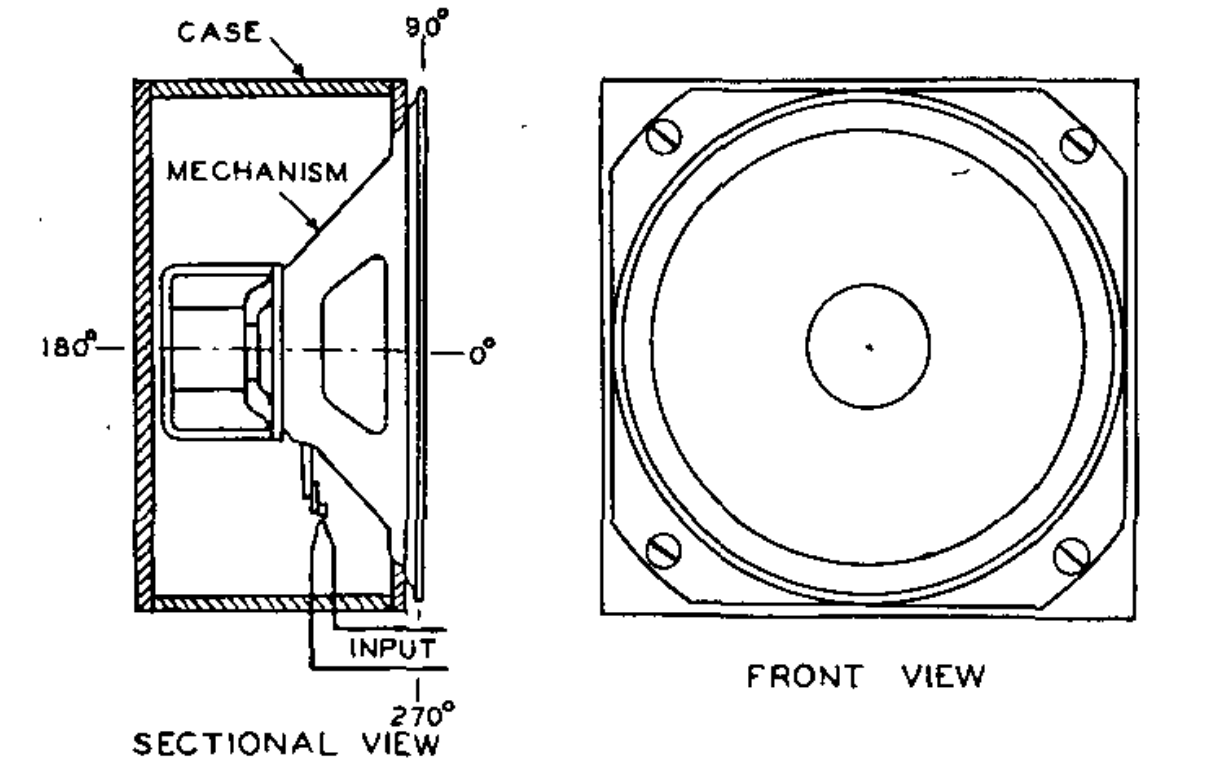
\includegraphics[scale=0.2]{figs/olsonFirstOrder.png}%
            \caption{Olson's first order unidirectional loudspeaker.}\cite{olson1973gradient}
            \label{olsonFirstOrderDiagram}
        \end{figure}
        Predating his work on gradient loudspeakers, Olson was an early descriptor of the beam narrowing effect of loudspeaker line arrays \cite{olson1957acoustical}.
        Line arrays would go on to be a principle tool of sound field control in the modern day.
        However, gradient loudspeakers are still, relative to line arrays, uncommon.
        Cardioid subwoofer systems used in live audio are common implementations of gradient loudspeaker designs.
        These subwoofers can be sold as gradient loudspeakers themselves, often with switchable directivity patterns; audio engineers will also arrange standard, omnidirectional subwoofers into configurations that introduce a phase delay sufficient to create a cardioid directivity pattern~\cite{curtis2022cardioidsubs}.
        Jordan Cheer elaborates on the use of a `two source line array', which in essence is an Olson-style directional gradient loudspeaker, stating: `Two-source line arrays have been used in a variety of applications to generate localised listening zones and have also been used as a constituent element of larger arrays to achieve sound field control more generally.'\cite{cheer2015robustness}.


    \section{Loudspeaker Construction}
        The prototype ACL has each low-frequency driver mounted in a shared, acoustically coupled enclosure.
        Robustness and efficiency of an acoustically coupled two-source superdirective array, an ICSV22 paper by Jordan Cheer, elaborates on the benefits of such a shared enclosure \cite{cheer2015robustness}.
        Cheer acknowledges how a superdirective array of loudspeakers have `high sensitivity to uncertainties in the assumed response of the system', and that regularization of the powered signal driving units in an array can improve the `robustness to uncertainty'.
        However, he further notes that these measures may limit the directivity of a such a system; counterproductive to the designed purpose of a superdirective array.
        Robustness and efficiency thus sets out to investigate the robustness of acoustically coupled two-source superdirective loudspeaker, as opposed to the previously investigated non-interacting directional loudspeakers.
        Cheer finds, using a two-port model of loudspeaker behavior and derived simulations, that an uncoupled two-source array is `more significantly affected by response uncertainties than the coupled array', and thus the coupled array is more robust, avoiding the need for regularization.
        \begin{figure}[H]
            \centering
            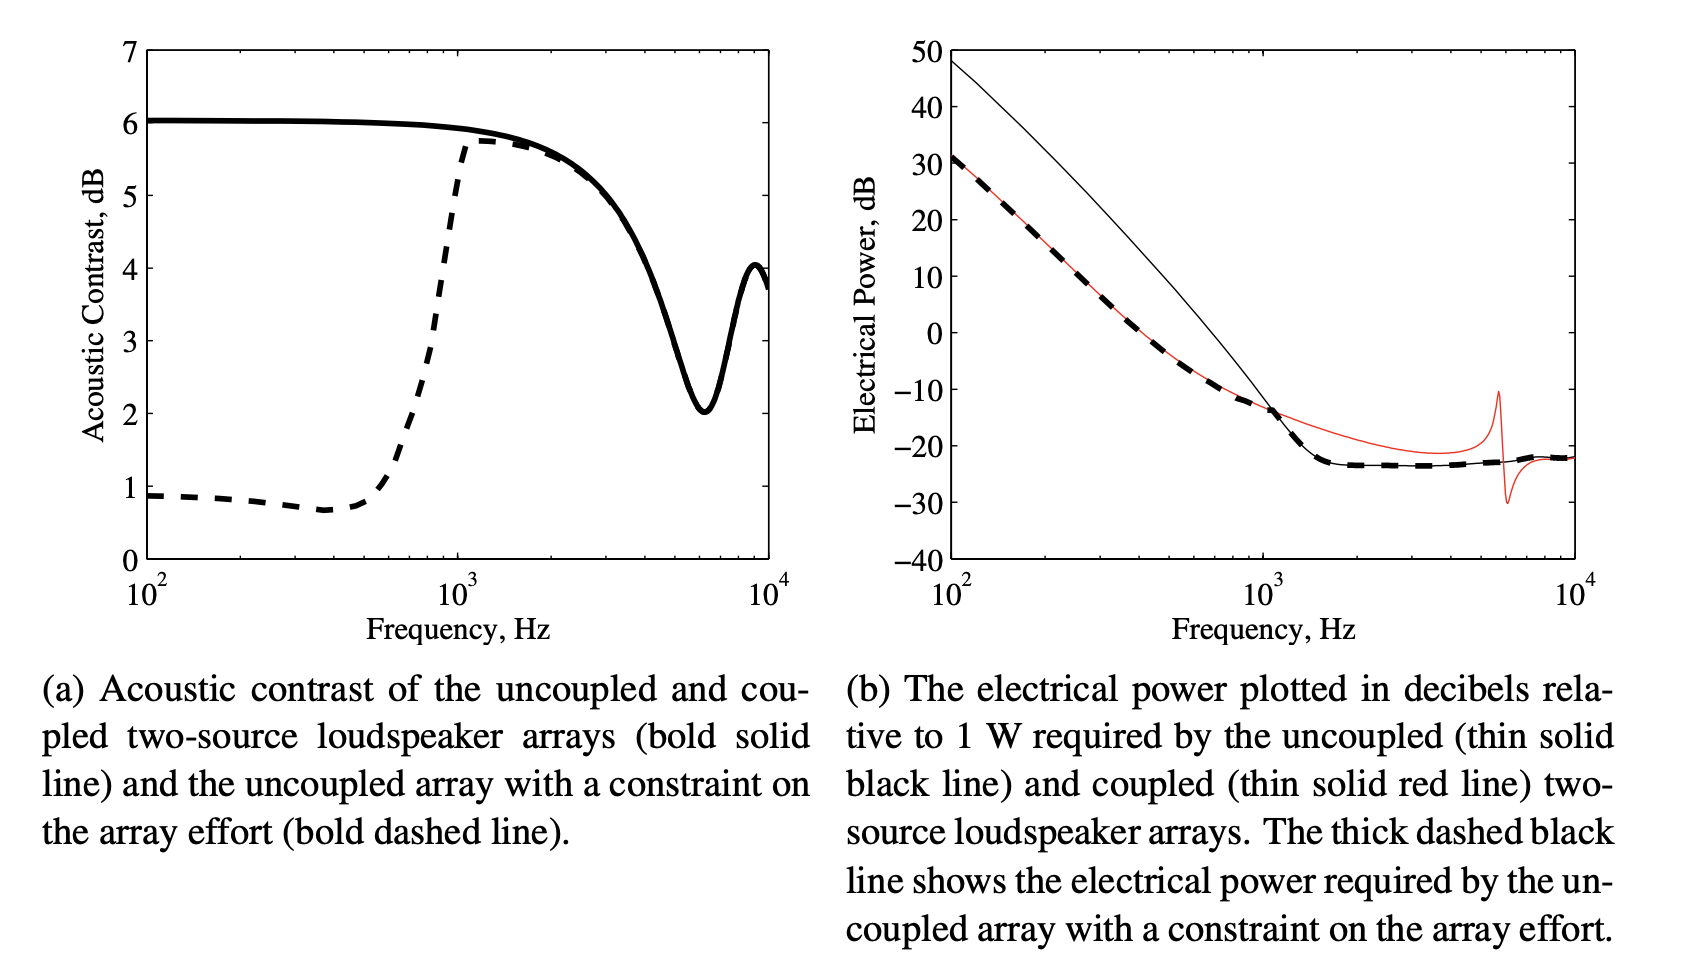
\includegraphics[scale=0.5]{figs/cheerGraph.png}%
            \caption{Cheer's plots comparing acoustically coupled and uncoupled loudspeaker systems.}\cite{cheer2015robustness}
            \label{cheerGraph}
        \end{figure}
        Cheer's figure \textit{a} (Fig.\ref{cheerGraph}) shows that when a constraint (to use the same electrical power as the coupled array) is applied to an \textit{un}-coupled two-source superdirective loudspeaker it loses a significant degree of acoustic contrast.


    \section{Quantifying Loudspeaker Directivity} 
        When describing a new, `holographic' near-field method of loudspeaker directivity measurement, Wolfgang Klippel and Christian Bellmann elaborate on the use of spherical harmonics as constituent solutions to the Helmholtz equation \cite{klippel2016holographic}.
        Whilst their paper focuses on the holographic directivity measurement method's effectiveness at reducing the space requirements of anechoic listening environments, the description of spherical harmonics
        
        The project described in this dissertation builds on previous work not only by the supervisory but also by other (former) students of the University of Salford.
        During the COVID-19 lock-down period the acoustic properties of the prototype loudspeaker were modelled with computer simulations.
        Paul Vedier carried out these simulations as part of his Master's dissertation.
        The spherical harmonic metric used by Vedier derived from Klippel's formulation.
        Vedier's paper confirms, using COMSOL, that the ACL has the properties of an Olson-style gradient loudspeaker.
        In Fig.\ref{vedierPolar} Vedier compares FEM analysis of two fully-modelled membranes in a cabinet and compares to Olson's analytical method.
        \begin{figure}[H]
            \centering
            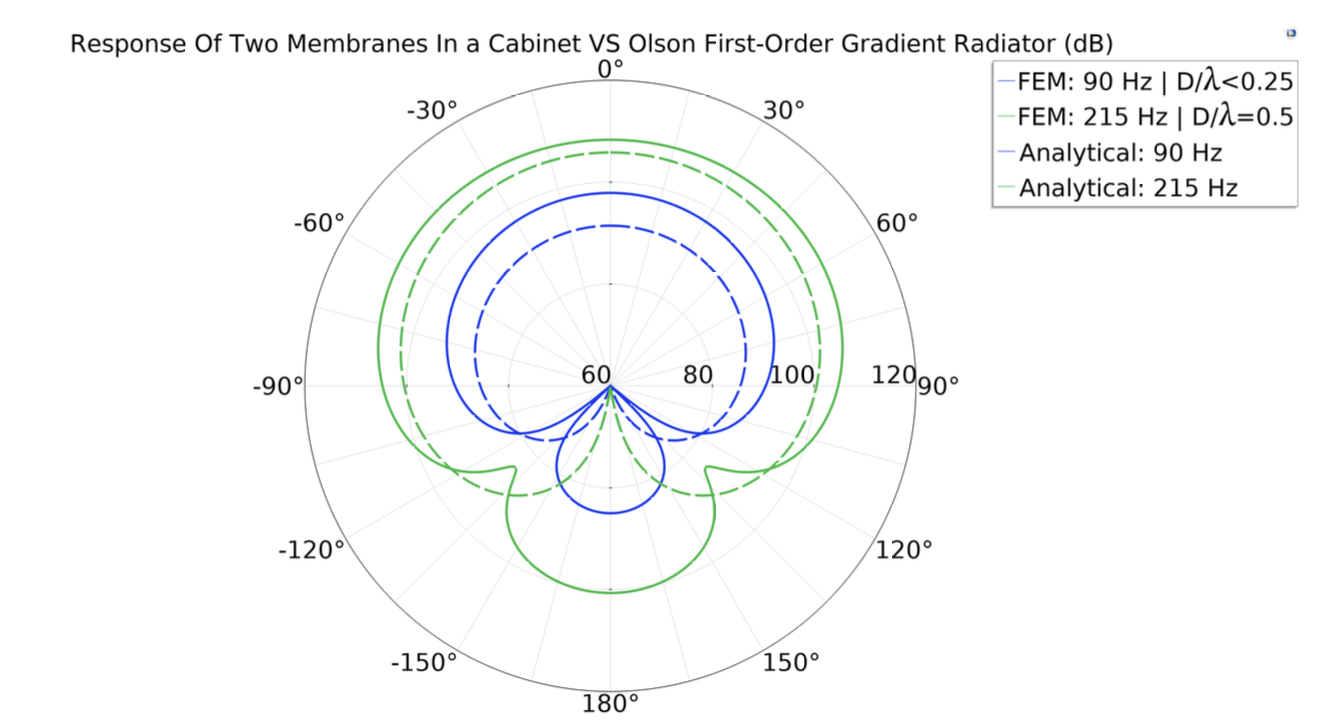
\includegraphics[scale=0.5]{figs/vedierPolar.png}
            \caption{FEM model of the ACL compared with Olson's first order unidirectional loudspeaker.}\cite{vedier}
            \label{vedierPolar}
        \end{figure}




    







\chapter{Key Theories}
    \section{Spherical Harmonics as a Method of Describing Cardioid Directivity}
    \section{Phase and Time Relationships Between Drivers}
    \section{Digital Signal Processing and Filtering}



\chapter{Methodology}
    \section{Initial Transfer Function and Directivity Measurement}
        SPEAKER WAS PUT IN THE ANECHOIC
        To build a numerical analysis of the directivity of the axisymmetric loudspeaker system's behavior as a whole over all frequencies, the frequency-domain transfer function of each driver must be measured across the entire X-Y AXIS MAYBE.
        In order to create a precise and accurate measurement free of interference and noise, the drivers were measured, mounted in the loudspeaker unit, in a fully anechoic chamber with a NTi reference-grade measurement mic.
        Ensuring the angle interval of each measurement was consistent, the loudspeaker was mounted to a Four Audio ELF robot arm which rotated the loudspeaker system about the X-Y AXIS MAYBE.
        Swept sine input signals were fed to each driver as the input excitation.
        The two low-frequency drivers were fed by a Samson SERVO-500 power amplifier, whilst the mid-high driver was fed by a University of Salford in-house made mono power amplifier, a 'Dial-a-Watt'.
        The output of the Dial-a-Watt was fed to a KEF-made cross-over, splitting the signal into mid and high frequency bands for the coaxial Uni-Q's mid and high drivers.
        The low frequency drivers had no cross-over filtering applied at this stage of the testing.
        The full signal flow of the transfer function measurement system is shown in Fig.\ref{signalFlow}.
        \begin{figure}[H]
            \centering
            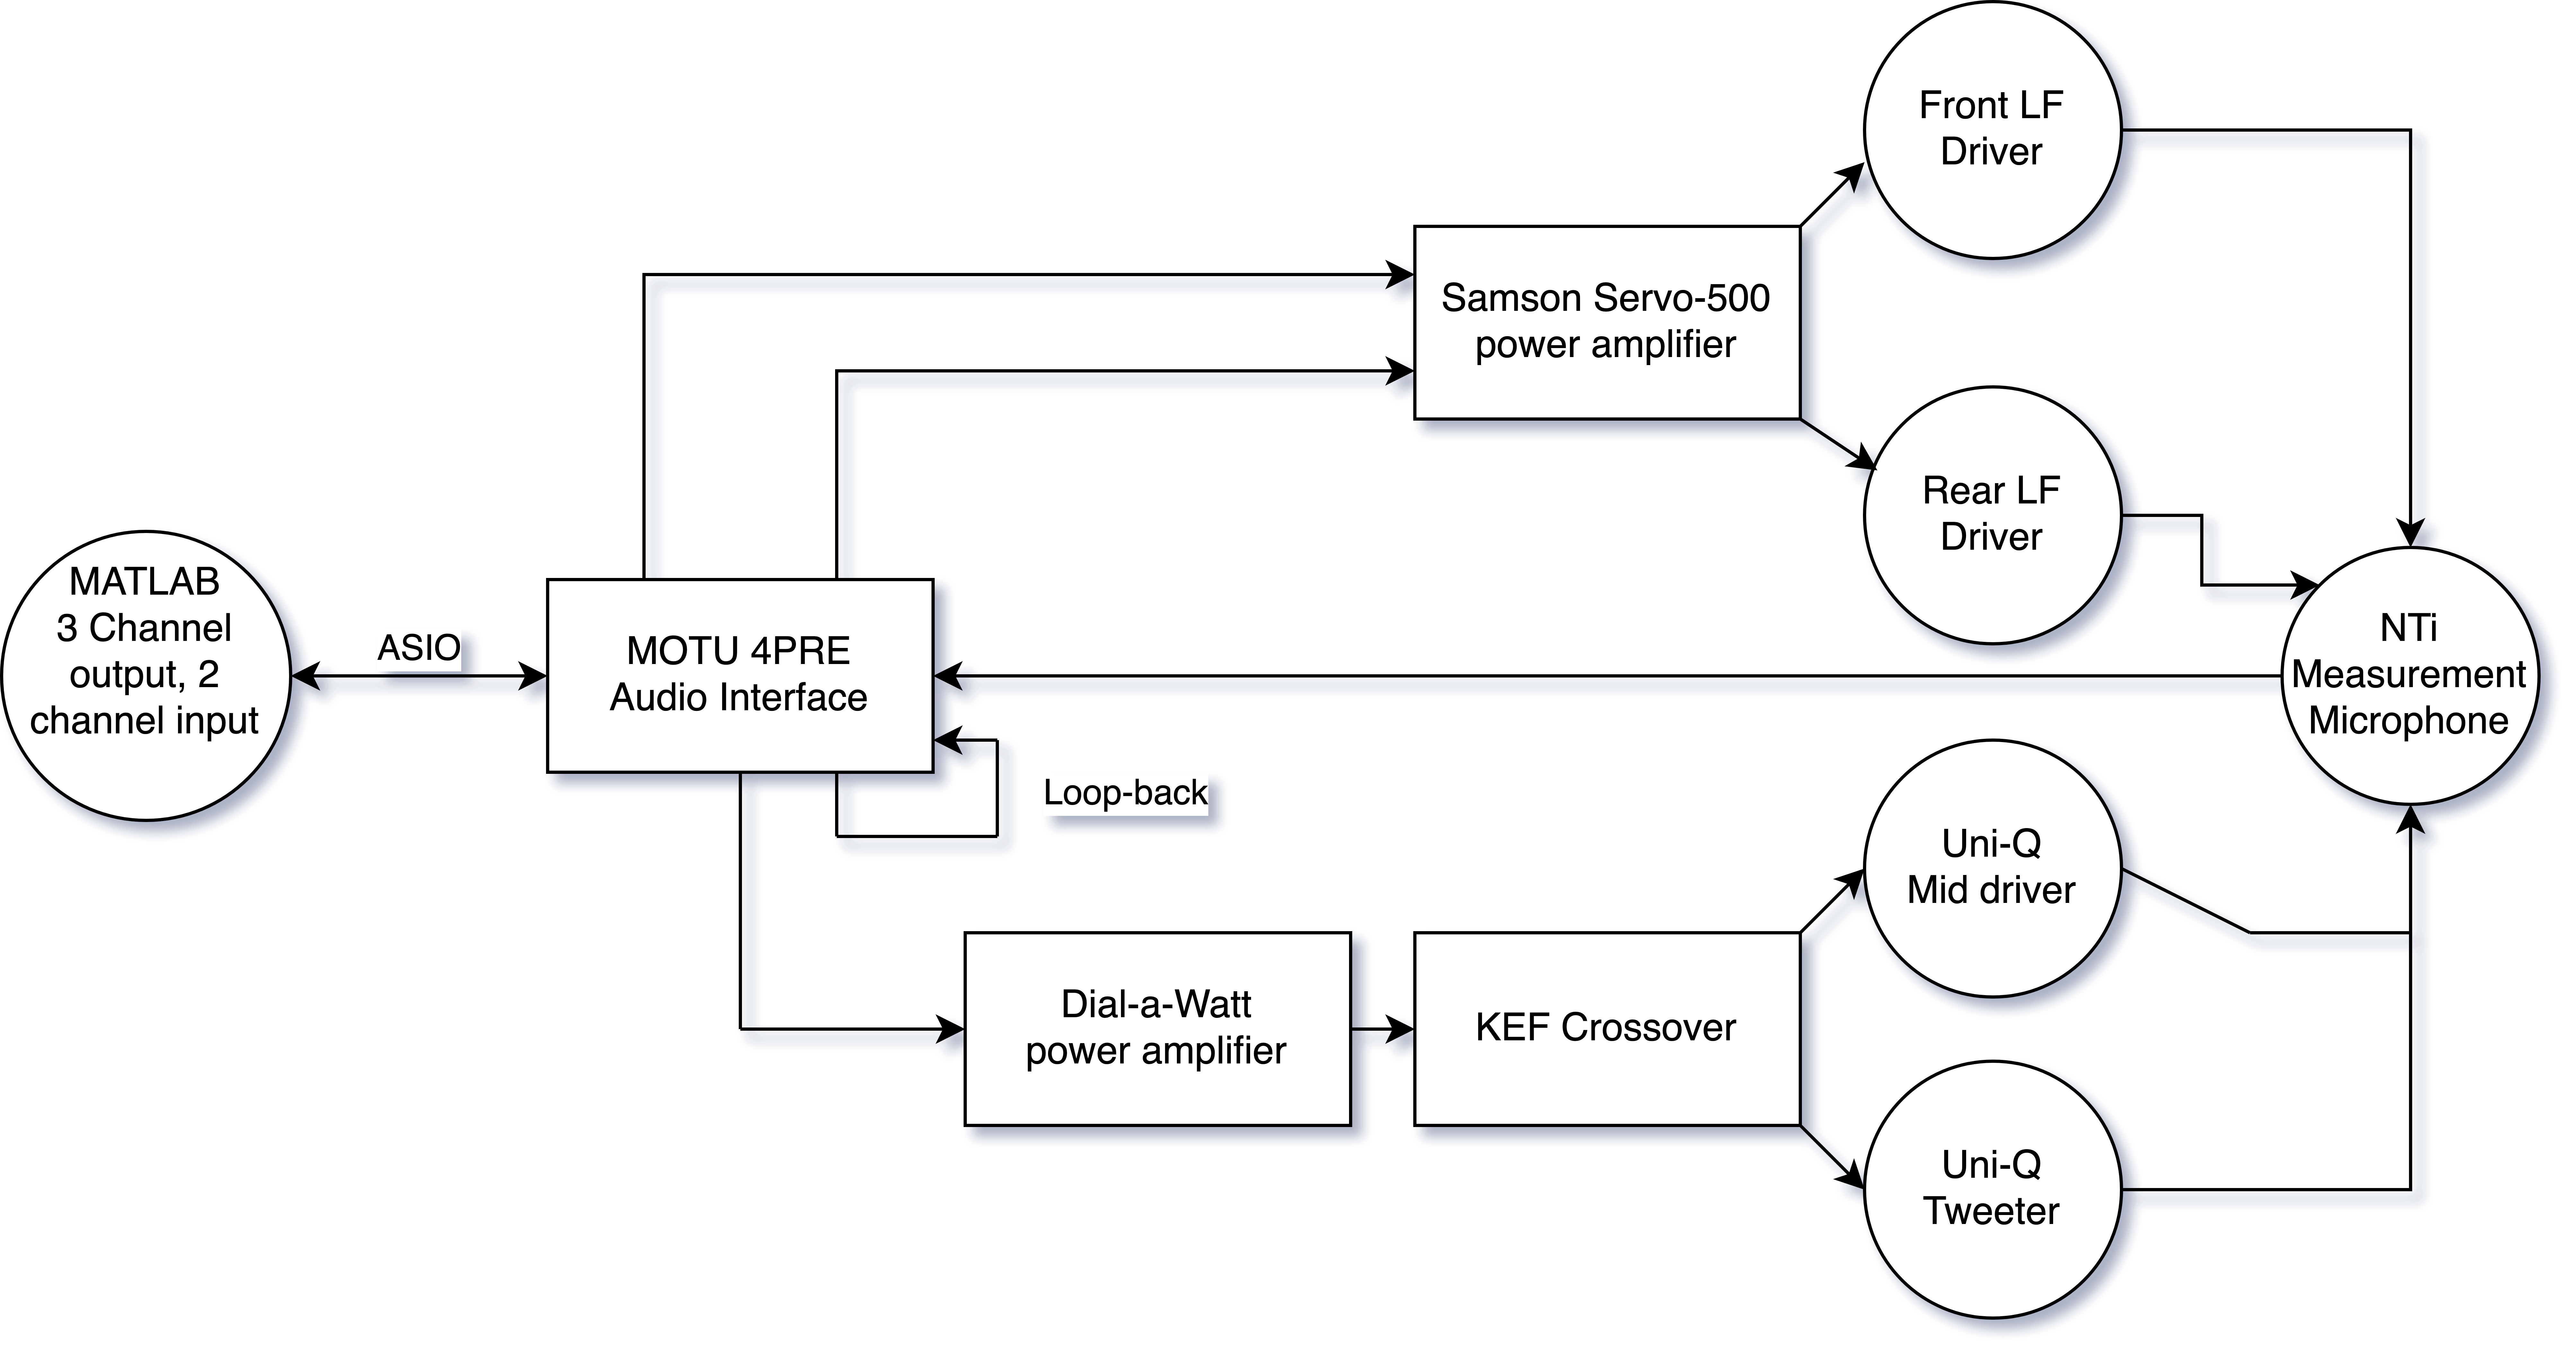
\includegraphics[scale=0.04]{figs/signalFlow.png}%
            \caption{Signal flow of driver transfer function measurement}
            \label{signalFlow}
        \end{figure}

        All audio output, robot arm movements and input recordings were automated through a MATLAB script.
        \begin{figure}[H]
            \centering
            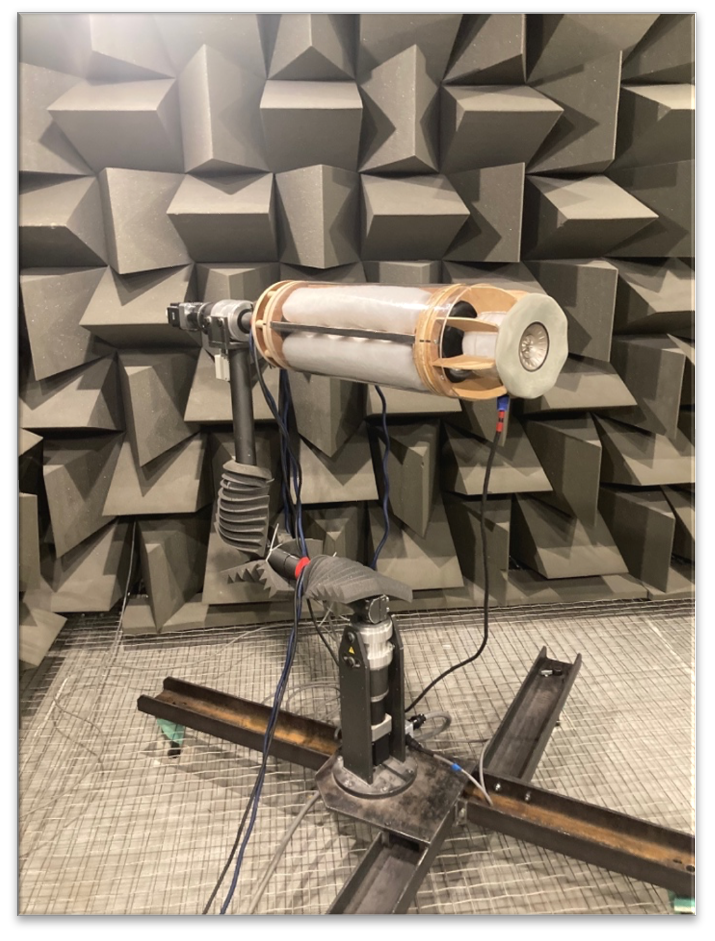
\includegraphics[scale=1]{figs/speakerOnRobot.png}%
            \caption{The prototype loudspeaker mounted for testing in the University of Salford's fully anechoic chamber.}
            \label{speakerOnRobot}
        \end{figure}
        A Bruel \& Kjaer measurement microphone placed 3.6m away was used to record relative sound pressure levels radiating from the loudspeaker drivers for each frequency at 121 angles.

        The raw results from this measurement were immediately processed; the dataset was large in file size and unwieldy to work with in MATLAB, so the data was reduced in size by taking only every 16th frequency point from the original, unnecessarily large frequency resolution.
        This had no apparent affect on the accuracy or validity of the measurements.
        Upon first inspection of the data, anomalous and invalid pressure-over-frequency data was found at a number of angles, shown in Fig.\ref{allAngles}.
        \begin{figure}[H]
            \centering
            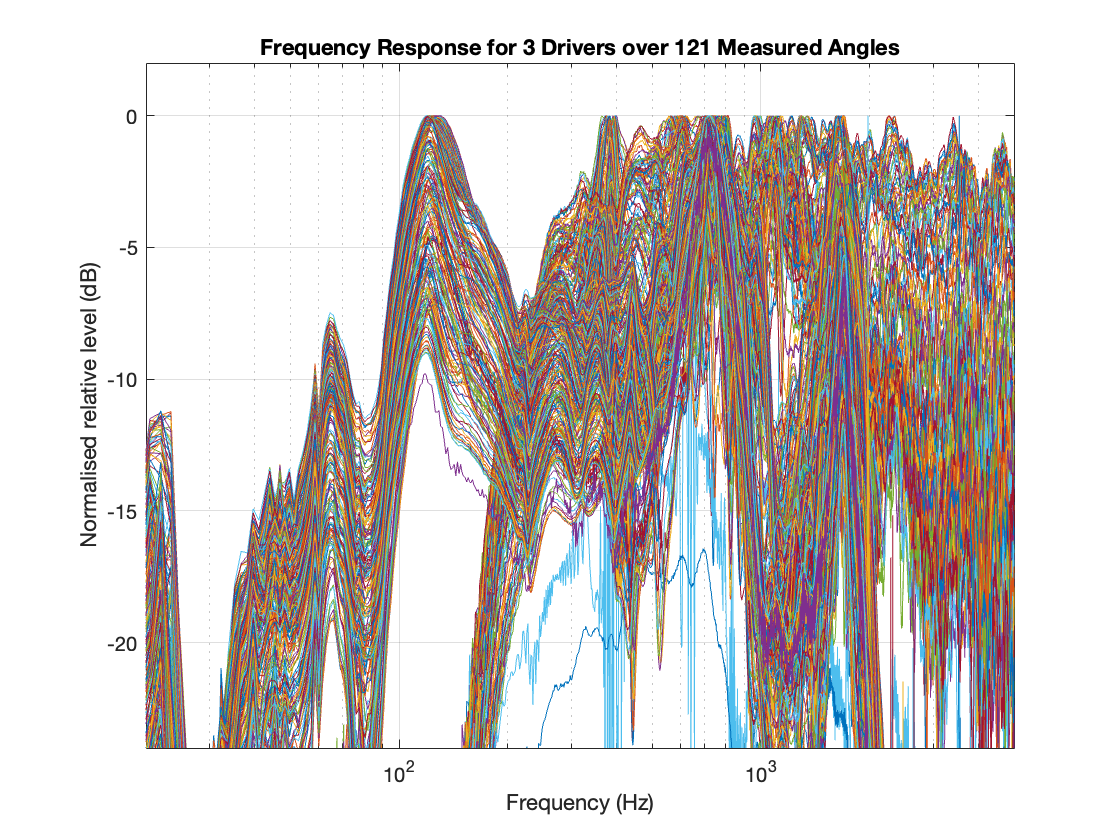
\includegraphics[scale=0.35]{figs/allAngles.png}%
            \caption{Noisy and anomalous data can be seen in the large blue and purple smears to the right. This data needed cleaning.}
            \label{allAngles}
        \end{figure}

    
    \section{Rear Driver Correction Filter Design}
        \section{Theory}
            The radiation of the rear driver of the ASL needs to have a particular phase relationship to radiation of the front driver.
            It is important to note that in order to maintain cardioid directivity across all frequencies, the frequency and directivity response of the rear driver in relation to the front driver must be accounted for.
            Using the metric of cardioid directivity given by Jonathan Hargreaves, previously used in Vedier's paper, a digital filter was used to encourage cardioid directivity across the working frequency range of the LF drivers CITE.
            When devising this metric, only the zeroth and first spherical harmonics were considered, as a true cardioid directivity can be described in three dimensions using only these harmonics ELABORATE MAYBE CITE.
            Using equation EQUATION HERE to find the coefficients $a_0$ and $a_1$ for the front and rear drivers.
            Equation \ref{sphericalPressure}.\ shows how spherical harmonic coefficients as a function of pressure over spherical angles, where the $R$ term accounts for any residual directivity.
            \begin{equation}
                p_{ff}(\beta,\alpha) = a_0 + a_1 \cos(\beta) + R(\beta,\alpha)
                \label{sphericalPressure}
                \cite{hargreaves}
            \end{equation}
            \begin{equation}
                \begin{split}
                    a_0(\omega) &= \frac{1}{ikh_0^{(1)}(kr_{meas})} \sqrt{\frac{1}{4\pi}} c_{0,0}(\omega) \\
                    a_1(\omega) &= \frac{1}{ikh_1^{(1)}(kr_{meas})} \sqrt{\frac{3}{4\pi}} c_{0,1}(\omega)
                    \label{a0a1}
                    \cite{hargreaves}
                \end{split}
            \end{equation}
            Equation \ref{a0a1} utilises Hankel functions, GOOD EXPLANATION AND CITATION HERE.
            The Hankel functions used are defined in Eq.\ref{hankel}
            \begin{equation}
                \begin{split}
                    h_0^1 &= -i  e^{ikr}  \frac{1}{kr} \\
                    h_1^1 &= -e^{ikr}  \frac{kr + i}{kr^2} ~\cite{hargreaves}
                    \label{hankel}
                \end{split}
            \end{equation}
            Conceptually, if the $a_0$ and $a_1$ coefficients are equal, the directivity pattern will be cardioid.
            It should be noted that the response of the $a$ coefficients above 500Hz is mostly irrelevant, as the LF drivers will be filtered out in favour of the Mid-High, which has a favourably cardioid directivity.

            The frequency magnitude response of the correction filter was derived by algebraically solving for $\gamma$ across the frequency-domain magnitude of each drivers $a_0$ and $a_1$ coefficients.
            \begin{equation}
                \gamma = \frac{a_{0f} - a_{1f}}{a_{1r} - a_{0r}}
            \end{equation}
            Each driver's $a_0$ and $a_1$ coefficients were derived using the initial frequency and directivity response measurements of the ASL.
            \begin{lstlisting}[style=Matlab-editor, gobble=16]
                function [a0, a1] = Compute_a_coeff(p, beta, k, r)
                    % Hankel functions (spherical bessel functions with decay):
                    h01 = -1i .* exp(1i .* k .* r) .* (1./(k.*r));
                    h11 = -exp(1i .* k .* r) .* (((k.*r) + 1i)./((k.*r).^2));

                    % Computing a_0, a_1 coefficients:
                    a0 = (pi./(2i .* k .* h01)) .* mean(p.*sin(beta),2);
                    a1 = ((3.*pi) ./ -(2.*k.*h11)) .* mean(p.*sin(beta).*cos(beta),2);
                
                end
            \end{lstlisting}
            Applying $\gamma$, the filter, to the rear LF woofer and recalculating the $a_0$ and $a_1$ coefficients for each driver gives a coefficient-over-frequency response shown in Fig.\ref{coeffsPredicted}.
            \begin{figure}[H]
                \centering
                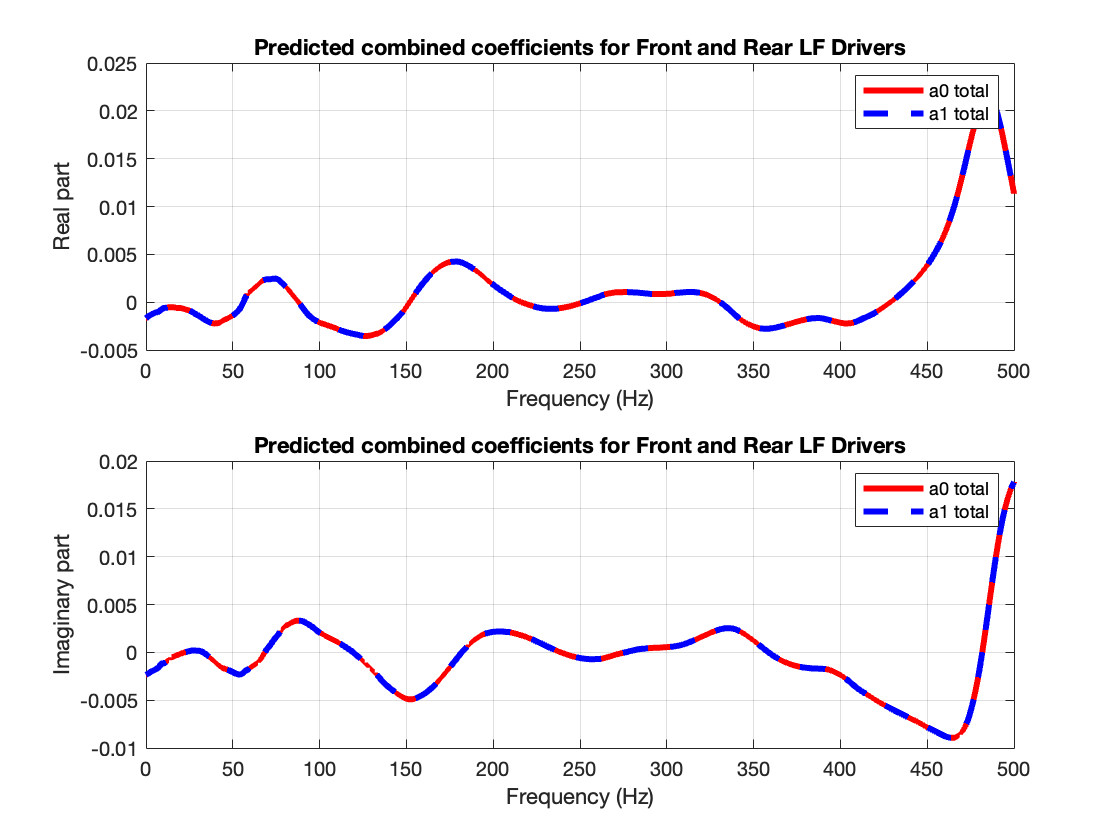
\includegraphics[scale=0.35]{figs/coeffsPredicted.png}%
                \caption{$a_0$ and $a_1$ coefficients remain equal across frequency after $\gamma$ is applied to the measured coefficients.}
                \label{coeffsPredicted}
            \end{figure}

        \section{Correction Filter Implementation}
            The generated impulse response, shown in Fig.\ref{origImpulse}, is non-causal, with a substantial section wrapped back around $t=0$ to the end of the response.
            This generated audible artifacts and ringing when convolved with any audio signal and played back.
            Thus, the impulse response of the filter was processed to eliminate this non-causality, but preserve it's original frequency and phase characteristics.
            Using MATLAB's \texttt(tukeywin()) function
            Gamma impulse response needed to be windowed around useful area, to shorten FIR filter and remove artifacts.


    \section{Measurement Revisited, Post Filtering}


\chapter{Discussion and Conclusions}

\chapter{Further Work}

\bibliographystyle{apalike}
\bibliography{theBib.bib}

\end{document}


